\documentclass[11pt,oneside]{scrbook}
\usepackage[a4paper,margin=2.4cm,marginparwidth=1.8cm,marginparsep=0.4cm]{geometry}
\usepackage{../common/rlstudy}

\title{{\color{rlblue}\textbf{Week 20}\\ \Huge GRPO, RLOO and RLVR:\\ critic-free RL for language models}}
\author{STUDY-RL --- a self-paced Deep RL curriculum}
\date{\today}

\begin{document}
\maketitle
\tableofcontents
\newpage

% ===========================================================================
\chapter*{Learning objectives}
\addcontentsline{toc}{chapter}{Learning objectives}


% Teaching companion: a small example before the full lecture.
\noindent\textbf{Study companion.} Read \texttt{teaching\_guide.md} in this
folder for step-by-step examples, an analogy with its limits, and self-checks.
Then use \texttt{workbook.ipynb} to implement and vary the calculations.
\par\medskip

\begin{keyidea}
By the end of this lecture you will be able to:
\begin{enumerate}\setlength{\itemsep}{2pt}
  \item Derive the REINFORCE-Leave-One-Out (RLOO) estimator from
        first principles and prove it is unbiased.
  \item Derive the GRPO group-relative advantage and explain why it is a
        control-variate variance-reduction technique.
  \item State the two debiasing fixes in Dr.~GRPO and the four upgrades in DAPO.
  \item Describe RLVR --- reinforcement learning with verifiable rewards ---
        and design a verifier for math, code, and tool use.
  \item Contrast process-reward models (PRMs) with outcome-reward models
        (ORMs), and cite the four leading PRM datasets.
  \item Implement a working GRPO loop on a verifiable-reward task from
        scratch and show held-out accuracy climbing during training.
  \item Articulate the central safety failure modes of RLVR (spec gaming
        the verifier, format hacking, distributional narrowing).
\end{enumerate}
\end{keyidea}

% ===========================================================================
\chapter{Motivation and intuition}

PPO is the workhorse of RLHF, but it carries an awkward passenger: the
\emph{critic}. A separate critic with a 7B-parameter backbone can add roughly
another 7B parameters; a small value head sharing the policy backbone does not.
The memory cost depends on this architecture and the training setup.
Token-level advantages require value estimates
trained on \emph{the policy's own distribution}, which drifts every step.

\marginnote{Shao et al. (2024) discuss the cost of a separate critic.}

Two 2024 papers study updates without a learned critic:
\textsc{Ahmadian et al., Back to Basics, arXiv:2402.14740} (RLOO) and
\textsc{Shao et al., DeepSeekMath, arXiv:2402.03300} (GRPO). Both observed
that completions in LLM RL are typically scored at the \emph{sequence} level
(``did the final answer match?''), so the credit-assignment problem PPO's
GAE was solving is largely a fiction. Replace the critic with a \emph{group
baseline}: sample $G$ completions per prompt, use their mean as the variance
reduction, and you keep almost all of PPO's stability at half the memory.

\begin{intuition}
Think of grading $G$ students on the same exam. Their mean score is a clean,
biased-free estimate of ``how hard the exam was'', so subtracting it from each
student's score isolates ``how well \emph{this} student did relative to the
class''. That isolated signal is your gradient. No instructor needs to predict
a student's score in advance (the value head); the class itself provides the
baseline.
\end{intuition}

The story then forks. \textbf{RLOO} keeps the sequence-level treatment
clean: one sample, one scalar advantage, one importance-weighted gradient.
\textbf{GRPO} broadcasts the advantage to every token and adds a PPO-style
clip plus KL-to-reference --- it is closer to ``critic-free PPO''. We will
derive both, and a 2025 debiasing patch (Dr.~GRPO, Liu et al.) that fixes a
length bias hiding inside GRPO's per-token normalisation.

Finally, the real point of this week is what these algorithms run \emph{on}:
\textbf{RLVR}, reinforcement learning with verifiable rewards. Math has
ground truth. Code has a unit-test executor. SAT-style logic has a checker.
Replace the reward model with a rule, and you get the recipe that produced
DeepSeek-R1, Kimi K1.5, Tülu-3 and Open-Reasoner-Zero in late 2024 and
early 2025.

% ===========================================================================
\chapter{Mathematical formulation}

\section{Why PPO became the wrong tool}

PPO was designed for continuous-control RL with three properties that
language modelling does \emph{not} share:

\begin{enumerate}\setlength{\itemsep}{2pt}
  \item \textbf{Dense per-step reward.} A walking robot earns a few units
        of reward every control step; an LLM earns one reward at the end of
        a 512-token generation. PPO's per-token advantage via GAE was
        solving a problem (smooth credit-assignment over hundreds of
        controls) that simply does not exist in the LLM setting.
  \item \textbf{Stationary state distribution.} A continuous-control
        environment hands you a stable state distribution to fit a value
        function against; an LLM generates its own context, so the value
        head is trying to fit a moving target every step.
  \item \textbf{Cheap rollouts.} Mujoco simulates a robot in microseconds.
        Generating a 512-token completion from a 7B model costs hundreds of
        milliseconds; the rollout cost vastly dominates the gradient cost,
        which inverts PPO's design trade-off between sample efficiency and
        gradient accuracy.
\end{enumerate}

The critic-free family replaces a learned baseline with one estimated from
other completions for the same prompt. With independent on-policy samples,
a leave-one-out baseline preserves the score-function gradient in expectation.
A mean including the current sample rescales that gradient; dividing by a
random group standard deviation changes prompt weighting as well.

\section{Setup: token-level MDP for a language model}

A prompt $x = x_{1:m}$ is fixed; the policy $\pi_\theta$ generates a
completion $y = y_{1:T}$ token by token, $y_t \sim \pi_\theta(\cdot \mid x,
y_{<t})$. A scalar reward $r(x, y) \in \Real$ is delivered at the end. The
RL objective is
\[
  J(\theta) \;=\; \E_{x \sim \mathcal{D},\; y \sim \pi_\theta(\cdot \mid x)}\!\big[r(x,y)\big].
\]
The policy-gradient theorem on this finite-horizon, terminal-reward MDP
yields
\begin{equation}\label{eq:pg}
  \nabla_\theta J(\theta) \;=\; \E_{x, y \sim \pi_\theta}\!\Big[\, r(x,y) \,\sum_{t=1}^{T}\nabla_\theta \log \pi_\theta(y_t \mid x, y_{<t})\,\Big].
\end{equation}

\begin{definition}[Score function]
$s_\theta(y_t; x, y_{<t}) \defeq \nabla_\theta \log \pi_\theta(y_t \mid x, y_{<t})$.
The factor $\sum_t s_\theta$ is the \emph{sequence-level score}.
\end{definition}

The only knob in this entire week is how we estimate $r(x,y) - b(\cdot)$ for
some baseline $b$ that does not depend on the sampled $y$.

\section{RLOO --- variance reduction by leave-one-out}

\begin{definition}[RLOO advantage]
Sample $G$ i.i.d.\ completions $y^{(1)},\dots,y^{(G)}$ from $\pi_\theta(\cdot \mid x)$
and score them, $r_i = r(x, y^{(i)})$. The RLOO advantage is
\[
  \hat A_i^{\text{RLOO}} \;=\; r_i \;-\; \frac{1}{G-1}\sum_{j \ne i} r_j
  \;=\; \frac{G}{G-1}\bigl(r_i - \bar r\bigr),
  \qquad \bar r = \tfrac{1}{G}\sum_j r_j.
\]
\end{definition}

\begin{theorem}[Unbiasedness of RLOO]\label{thm:rloo-unbiased}
For $G\ge2$ independent on-policy samples from $\pi_\theta$, a parameter-independent reward, and integrable score-weighted rewards, $\E[\hat A_i^{\text{RLOO}} \, s_\theta(y^{(i)})] = \nabla_\theta J(\theta)$.
\end{theorem}

\begin{proof}
The leave-one-out baseline $b_i \defeq \tfrac{1}{G-1}\sum_{j \ne i} r_j$ is
a deterministic function of $\{y^{(j)}\}_{j \ne i}$ and is therefore
independent of $y^{(i)}$ under i.i.d.\ sampling. Hence
$\E[b_i \, s_\theta(y^{(i)})] = \E[b_i] \cdot \E[s_\theta(y^{(i)})]$, and the
expected score is zero (the score-function identity:
$\E_{y \sim \pi}[\nabla \log \pi(y)] = \nabla \sum_y \pi(y) = 0$). The first
term gives the policy gradient~\eqref{eq:pg}. $\Box$
\end{proof}

\begin{theorem}[Variance-optimal constant baseline]
\label{thm:rloo-varred}
Let $S(y)=\nabla_\theta\log\pi_\theta(y\mid x)$ denote the sequence score.
For a constant baseline $b$, finite second moments, and $\E[\|S\|^2]>0$,
the baseline minimising the trace of the gradient covariance is
\[
 b^\star=\frac{\E[r\|S\|^2]}{\E[\|S\|^2]}.
\]
This equals $\E[r]$ only when the reward and squared score norm have
zero covariance. A random leave-one-out estimate also introduces baseline
estimation noise, so it is not guaranteed to beat no-baseline REINFORCE.
\end{theorem}
\begin{proof}
The gradient mean $g=\E[(r-b)S]=\E[rS]$ does not depend on $b$.
Thus the covariance trace is $\E[(r-b)^2\|S\|^2]-\|g\|^2$.
Differentiate with respect to $b$, set the result to zero, and solve.
\end{proof}
\begin{pitfall}
Variance of reward coefficients alone is not variance of policy gradients.
Multiplying by different score vectors changes both magnitude and direction.
Even under reward--squared-score independence, an individual RLOO term has
$\E[(r-b_i)^2]=\mathrm{Var}(r)G/(G-1)$, which need not be smaller than
$\E[r^2]$. The covariance between terms also matters when averaging a group.
\end{pitfall}

\section{GRPO --- group-relative normalised advantage}

\begin{definition}[GRPO advantage]
Given the same group $\{r_1,\dots,r_G\}$,
\[
  \hat A_i^{\text{GRPO}} \;=\; \frac{r_i - \bar r}{\sigma_r + \varepsilon},
  \qquad \sigma_r^2 = \tfrac{1}{G}\sum_j (r_j - \bar r)^2.
\]
\end{definition}

\marginnote{The $\sigma_r$ divisor normalises the advantage to roughly unit
variance per group --- handy for a single global learning rate across very
different prompts.}

Plug $\hat A_i$ into a PPO-clipped surrogate, broadcast to every token,
and add a KL-to-reference:
\begin{equation}\label{eq:grpo}
\begin{aligned}
  \mathcal{L}_{\text{GRPO}}(\theta)
  &= -\E_{x, \{y^{(i)}\}}\!\Bigg[\frac{1}{G}\sum_{i=1}^{G}\frac{1}{|y^{(i)}|}\sum_{t=1}^{|y^{(i)}|}\!\Big( \min(\rho_{i,t}\hat A_i,\, \mathrm{clip}(\rho_{i,t}, 1\!-\!\varepsilon, 1\!+\!\varepsilon)\hat A_i) \\[-2pt]
  &\hspace{8.5em}-\, \beta\, \KL_{i,t}\big[\pi_\theta \,\|\, \pi_{\text{ref}}\big] \Big)\Bigg],
\end{aligned}
\end{equation}
where $\rho_{i,t} = \pi_\theta(y_t^{(i)} \mid \cdot) / \pi_{\theta_{\text{old}}}(y_t^{(i)} \mid \cdot)$
is the per-token importance ratio.

\begin{theorem}[GRPO advantage is mean-zero by construction]
$\sum_i \hat A_i^{\text{GRPO}} = 0$ for every group. This is a coefficient identity, not a guarantee about group probability:
score vectors, token lengths, clipping, and shared parameters also affect the update.
\end{theorem}

\begin{proof}
$\sum_i (r_i - \bar r) = 0$ by definition of $\bar r$, and dividing by
$\sigma_r + \varepsilon$ preserves zero sum. $\Box$
\end{proof}

\subsection*{Dr.\,GRPO --- removing the length and difficulty biases}

\textsc{Liu et al., 2025, arXiv:2503.20783} identify two biases hiding in
the GRPO loss~\eqref{eq:grpo}:

\begin{enumerate}\setlength{\itemsep}{2pt}
  \item \textbf{Length bias.} Multiplying by $1/|y^{(i)}|$ gives each token in a longer response a smaller coefficient. This changes relative sequence weighting; its effect on length depends on reward sign and the correlation between length and correctness.
  \item \textbf{Difficulty bias.} Dividing by $\sigma_r$ \emph{amplifies}
        gradients on prompts where the group has small intra-variance
        (near-uniform but mixed rewards) relative to higher-variance groups.
        Exactly uniform rewards give zero centred advantages, so their reward
        gradient is zero even when the standard deviation is zero.
\end{enumerate}

The Dr.~GRPO patch is two lines: \texttt{(i)} drop the $1/|y|$ divisor (sum
the token losses, do not average them); \texttt{(ii)} use the un-normalised
advantage $r_i - \bar r$ (or normalise across the dataset, not the group).
Empirically these two patches alone produce a noticeable jump in MATH
accuracy and \emph{shorter}, not longer, chains of thought.

\begin{pitfall}
The Dr.~GRPO fixes are also a good cautionary tale: the original GRPO loss
\emph{looks} like the natural per-token cross-entropy formulation a deep
learning practitioner would write. The bug was invisible until the team
ran a careful length/difficulty diagnostic. Always plot the distribution
of completion lengths during RL training.
\end{pitfall}

\subsection*{DAPO --- four upgrades for production-scale GRPO}

\textsc{Yu et al., DAPO, arXiv:2503.14476} stack four further tricks on top
of GRPO:

\begin{itemize}\setlength{\itemsep}{2pt}
  \item \emph{Clip-Higher}: asymmetric clip $\varepsilon_\text{low} \ne \varepsilon_\text{high}$,
        usually $0.2$ versus $0.28$. Lets low-probability exploration tokens
        get probability mass without being capped on the upside.
  \item \emph{Dynamic Sampling}: discard prompts whose group accuracy is $0$
        or $1$ (they yield zero advantage and waste gradient capacity).
  \item \emph{Token-level loss}: aggregate over valid tokens across the batch. This differs from Dr.~GRPO\textquotesingle s fixed normalisation; both remove per-response length denominators.
  \item \emph{Overlong reward shaping}: a soft penalty on completions that
        hit the truncation budget, preventing catastrophic gradient spikes
        when the policy starts ``thinking out loud forever''.
\end{itemize}

\section{ReMax and VinePPO in one paragraph each}

\textbf{ReMax} (\textsc{Li et al., arXiv:2310.10505}) replaces the LOO/group
baseline with the \emph{greedy} reward $r^\text{greedy}$: deterministic
decode once, use that as a constant baseline. One extra forward, no value
net, and very low variance whenever the greedy decode is informative ---
which is most of the time for instruction-following RLHF.

\textbf{VinePPO} (\textsc{Kazemnejad et al., arXiv:2410.01679}) goes the
other way: keep PPO's per-token credit assignment, but estimate $V(s)$ on
the fly with $K$ short Monte-Carlo rollouts (``vines'') branched from
every prefix. Eliminates the learned critic, gives per-step process
rewards, and converges with $9\times$ fewer iterations than PPO on MATH.
The price is the extra rollouts.

\section{RLVR --- reinforcement learning with verifiable rewards}

\begin{definition}[Verifiable-reward task]
A task is \emph{verifiable} when there exists a deterministic rule
$\text{verify}\colon (x, y) \mapsto \{0, 1\}$ that returns $1$ iff $y$
contains the right answer (or runs cleanly through a code sandbox, or
passes a formal proof checker).
\end{definition}

The standard ingredients of an RLVR recipe (DeepSeek-R1, Tülu-3,
Open-Reasoner-Zero):

\begin{enumerate}\setlength{\itemsep}{2pt}
  \item A \textbf{rule reward} --- exact-match on the final number,
        symbolic-equivalence via \texttt{sympy}, unit tests in a sandboxed
        executor.
  \item Optional \textbf{format reward} --- $+0.1$ if the completion
        contains \verb|<think>...</think>| tags or a \verb|####|-prefixed
        final answer. Watch out: this is the most common reward hack
        surface in RLVR.
  \item A \textbf{KL anchor} to the SFT initialisation, often with
        $\beta = 0.01$--$0.04$, sometimes dropped entirely (Open-Reasoner-Zero
        argues KL is unnecessary on verifiable tasks; R1-Zero agrees).
  \item A critic-free policy gradient --- GRPO or RLOO --- with $G = 8$--$16$.
\end{enumerate}

\subsection*{Verifier design}

For math, the canonical pipeline is: \texttt{(1)} strip the completion to
the last line; \texttt{(2)} extract via regex \verb|####\s*(-?[\d./]+)|;
\texttt{(3)} pass the candidate and ground truth through \texttt{sympy.simplify}
and accept iff their difference is zero. For code, \texttt{(1)} parse out a
\verb|```python|-fenced block; \texttt{(2)} run it against unit tests inside
a \texttt{seccomp}/\texttt{firejail} sandbox with a 5\,s wall-clock; \texttt{(3)}
reward $1$ iff all tests pass. For tool use, the verifier inspects the
sequence of tool calls and matches against an oracle trace; partial credit
is risky and often hacked.

\section{Process rewards vs outcome rewards}

\begin{definition}[ORM]
An \emph{outcome reward model} returns a scalar on the full $(x, y)$ pair
and ignores intermediate steps. Exact-match is an ORM.
\end{definition}

\begin{definition}[PRM]
A \emph{process reward model} returns a scalar per step
$r(x, y_{1:t})$ for every $t$. The trajectory reward is then aggregated ---
typically as the minimum, the mean, or a product of step probabilities.
\end{definition}

Four PRM datasets dominate the literature:

\begin{itemize}\setlength{\itemsep}{2pt}
  \item \textsc{PRM800K} (\textsc{Lightman et al., 2023, arXiv:2305.20050})
        --- 800K human step labels on MATH. First showed PRMs beat ORMs at
        best-of-N re-ranking on MATH.
  \item \textsc{Math-Shepherd} (\textsc{Wang et al., 2024, arXiv:2312.08935})
        --- automatic step labels via Monte-Carlo rollouts; a step is
        ``good'' iff continuing from it disproportionately reaches the
        correct final answer.
  \item \textsc{OmegaPRM} (\textsc{Luo et al., 2024, arXiv:2406.06592}) ---
        MCTS-based automatic PRM data generation. Drove Gemini's math gains.
  \item \textsc{GenRM} (\textsc{Zhang et al., 2024, arXiv:2410.12832}) ---
        reward is the probability of the token ``yes'' under a judge LLM
        prompted with a rubric. \textsc{Rubric-RM / OpenRubrics}
        (\textsc{arXiv:2510.07743, 2025}) extends this with synthetic
        rubrics.
\end{itemize}

\begin{intuition}
PRMs shine when the search space is large and pruning early matters ---
MCTS, beam search, best-of-N over long chains. ORMs win on RLVR with cheap
exact-match: the marginal accuracy gain of step labels rarely justifies
the labelling cost and they enlarge the reward-hacking surface (every step
becomes a place to game).
\end{intuition}

\section{The KL anchor: what it does and when to drop it}

The KL-to-reference term $\beta \, \KL(\pi_\theta \,\|\, \pi_\text{ref})$
serves three purposes that are worth distinguishing:

\begin{enumerate}\setlength{\itemsep}{2pt}
  \item \textbf{Trust region.} It prevents the policy from drifting so far
        in one step that the importance ratio $\rho$ explodes and the
        clipped surrogate degenerates. PPO's clip does some of this job
        already; the KL term is the safety net.
  \item \textbf{Prior preservation.} It anchors the policy near a known-good
        reference (the SFT model). This is essential in preference-RLHF
        where the reward model is itself fit only locally; if the policy
        wanders into reward-model out-of-distribution territory, you have
        no guarantee the reward signal is meaningful.
  \item \textbf{Skill retention.} It implicitly fights catastrophic
        forgetting of non-rewarded skills. The SFT model knew how to do
        creative writing and dialogue; pure RLVR shrinks that distribution.
\end{enumerate}

For \emph{verifiable} tasks (purposes 1 and 3 only), \textsc{Open-Reasoner-Zero}
and \textsc{R1-Zero} report that the KL term is essentially dispensable
when the base model is strong enough: the reward signal is grounded in
external truth, so there is no out-of-distribution risk on the reward
side, and the clip alone provides the trust region. For
\emph{preference} RLHF (purpose 2), removing the KL anchor reliably
explodes the policy into reward-model artifacts within tens of steps.

For samples from $p$ with common positive support for $p$ and $q$, define
\[
 \hat k^3=e^{\log q-\log p}-(\log q-\log p)-1.
\]
Since $\E_p[q/p]=1$, $\E_p[\hat k^3]=\KL(p\|q)$.
The sample is non-negative because $e^u\ge1+u$.
Its variance can be lower near $p=q$; this is not a universal variance bound.
If samples instead come from an older policy, the same unweighted average
is not generally an unbiased estimate of the current-policy KL.

\begin{pitfall}
The signed estimator $\log p-\log q$ is valid in expectation under $p$;
a negative sample is not a bug. Also distinguish an unbiased scalar KL
estimate from its gradient: differentiating an estimate while treating
samples as fixed omits the derivative of the sampling distribution.
Choose reward shaping, an exact categorical KL, or a documented surrogate
with the appropriate sampling/importance-weight convention.
\end{pitfall}

\section{Empirical variance scaling}

\begin{figure}[t]
\centering
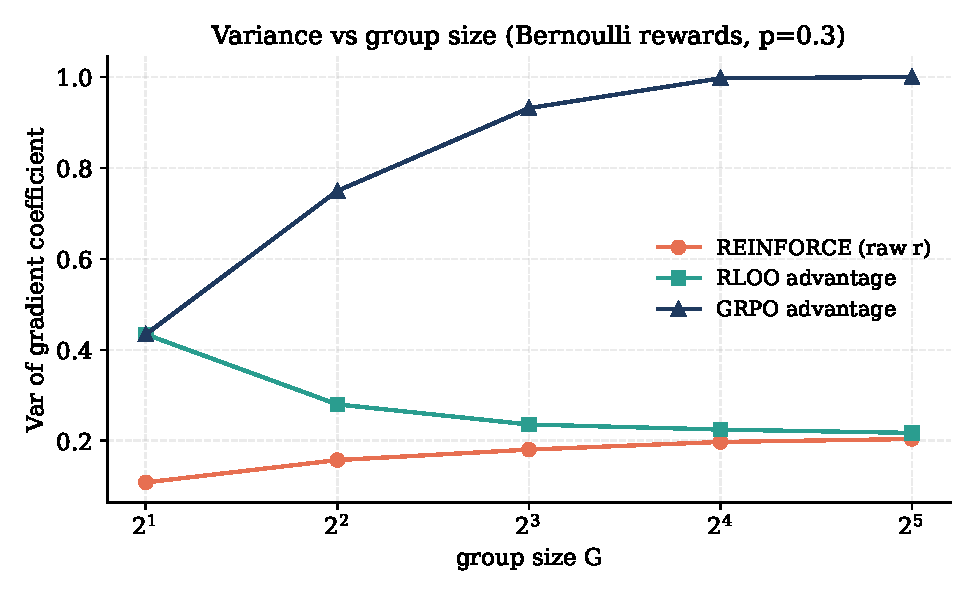
\includegraphics[width=0.7\linewidth]{figs/fig_variance.pdf}
\caption{Variance of the gradient coefficient under three estimators as
group size grows. Bernoulli rewards with $p=0.3$. RLOO and GRPO are both
group-baseline control variates; GRPO additionally divides by group
$\sigma_r$, which on this Bernoulli case happens to inflate variance for
mid-sized groups before settling. The plot motivates the Dr.~GRPO debias.}
\label{fig:variance}
\end{figure}

% ===========================================================================
\chapter{Algorithms}

\begin{tcolorbox}[colback=rlbg,colframe=rlblue,title={Algorithm: GRPO step (DeepSeekMath, 2024)}]
\textbf{Input.} prompt $x$, group size $G$, current policy $\pi_\theta$,
reference policy $\pi_\text{ref}$, KL coefficient $\beta$, clip $\varepsilon$.\\[2pt]
\textbf{1.} Sample $G$ completions $\{y^{(i)}\}$ from $\pi_{\theta_\text{old}}(\cdot \mid x)$.\\
\textbf{2.} Compute rewards $r_i = r(x, y^{(i)})$ via the verifier.\\
\textbf{3.} Form group baseline $\bar r$ and (optionally) $\sigma_r$;
   compute $\hat A_i = (r_i - \bar r)/(\sigma_r + \varepsilon)$.\\
\textbf{4.} For every token in every $y^{(i)}$, compute the importance ratio
   $\rho_{i,t}$ and the unbiased KL estimate
   $\hat k^3_{i,t} = e^{\log\pi_\text{ref} - \log\pi_\theta} - (\log\pi_\text{ref} - \log\pi_\theta) - 1$.\\
\textbf{5.} Form the clipped surrogate~\eqref{eq:grpo}, take an Adam step,
   clip gradient norm.
\end{tcolorbox}

\begin{tcolorbox}[colback=rlbg,colframe=rlblue,title={Algorithm: RLOO step (Ahmadian et al., 2024)}]
\textbf{Input.} prompt $x$, group size $G$, current policy $\pi_\theta$.\\[2pt]
\textbf{1.} Sample $G$ completions $\{y^{(i)}\}$ from $\pi_\theta(\cdot \mid x)$,
caching their on-policy log-probs.\\
\textbf{2.} Compute rewards $r_i = r(x, y^{(i)})$ via the verifier.\\
\textbf{3.} Form per-sample LOO baselines
$b_i = \frac{1}{G-1}\sum_{j \ne i} r_j$ and advantages $\hat A_i = r_i - b_i$.\\
\textbf{4.} Treat each completion as a single action with sequence-level
log-probability $\log \pi_\theta(y^{(i)} \mid x) = \sum_t \log \pi_\theta(y_t^{(i)} \mid \cdot)$.\\
\textbf{5.} Loss $\mathcal{L} = - \tfrac{1}{G}\sum_i \hat A_i \log \pi_\theta(y^{(i)} \mid x)$.\\
\textbf{6.} Optional: PPO clip on the sequence-level importance ratio if you
multi-step the same batch.
\end{tcolorbox}

\begin{tcolorbox}[colback=rlbg,colframe=rlblue,title={Algorithm: Dr.GRPO step (Liu et al., 2025)}]
\textbf{Input.} as for GRPO, plus the debiased flag.\\[2pt]
\textbf{1--2.} Identical to GRPO.\\
\textbf{3.} Form $\hat A_i = r_i - \bar r$ \emph{(no division by $\sigma_r$)}.\\
\textbf{4--5.} Identical to GRPO clipped surrogate.\\
\textbf{6.} Token loss is \emph{summed} over tokens, not averaged
(removes the $1/|y|$ length bias).\\
\textbf{7.} Mean over sequences in the batch (yes), Adam step, clip grad norm.
\end{tcolorbox}

\subsection*{Worked numerical example}

A single prompt $x = $ ``$3+4=$''. Sample $G = 4$ completions:
$y^{(1)} = $ ``$7$\verb|<eos>|'' ($r_1 = 1$),
$y^{(2)} = $ ``$5$\verb|<eos>|'' ($r_2 = 0$),
$y^{(3)} = $ ``$7$\verb|<eos>|'' ($r_3 = 1$),
$y^{(4)} = $ ``=='' ($r_4 = 0$, no number found).

$\bar r = 0.5$, $\sigma_r = 0.5$. GRPO advantages
$\hat A = (1, -1, 1, -1)$ (unit normalised). RLOO advantages
$\hat A^{\text{RLOO}} = \frac{4}{3}(0.5, -0.5, 0.5, -0.5) = (\tfrac{2}{3}, -\tfrac{2}{3}, \tfrac{2}{3}, -\tfrac{2}{3})$.
Dr.~GRPO advantages
$\hat A^{\text{Dr}} = (0.5, -0.5, 0.5, -0.5)$.

Notice: all three estimators give exactly the same \emph{sign} on every
sample. The differences are scale (which the learning rate absorbs) and
the implicit weighting between prompts with high vs low intra-variance
(which Dr.~GRPO targets).

\subsection*{Complexity}

Per GRPO step on a sequence of length $T$, group size $G$, prompts $P$:
$\mathcal{O}(PG \cdot T \cdot d^2)$ forward, identical backward; the
verifier adds $\mathcal{O}(PG)$ regex evaluations (negligible) or
sandboxed execution (dominant if you use code rewards).

% ===========================================================================
\chapter{Implementation walkthrough}

The mini-project lives under \texttt{project/}. Three files matter:
\texttt{env.py} (toy arithmetic + verifier), \texttt{agent.py} (a tiny
$\sim 30$k-parameter char-level Transformer), and \texttt{train.py} (the
GRPO loop with RLOO and Dr.~GRPO switches). On a single CPU thread, the
full train converges in $\sim 15$\,s.

\section{The verifier}

\begin{minted}[fontsize=\footnotesize]{python}
_NUM_RE = re.compile(r"-?\d+")

def extract_final_number(text):
    matches = _NUM_RE.findall(text)
    if not matches:
        return None
    try:
        return int(matches[-1])
    except ValueError:
        return None

def exact_match_reward(completion, target):
    pred = extract_final_number(completion)
    return 1.0 if pred is not None and pred == target else 0.0
\end{minted}

That is the entire RLVR reward for this week. Note the explicit guard
against ``no number found'' --- a model that emits only \texttt{====} would
otherwise compare \texttt{None == target} and crash, or worse, silently
match \texttt{None == None} on some Python paths.

\section{The advantage estimators}

\begin{minted}[fontsize=\footnotesize]{python}
def grpo_advantages(rewards, eps=1e-6, debias=False):
    mean = rewards.mean(dim=-1, keepdim=True)
    if debias:                            # Dr.GRPO
        return rewards - mean
    std = rewards.std(dim=-1, keepdim=True, unbiased=False)
    return (rewards - mean) / (std + eps)

def rloo_advantages(rewards):
    G = rewards.shape[-1]
    mean = rewards.mean(dim=-1, keepdim=True)
    return (G / (G - 1)) * (rewards - mean)
\end{minted}

\section{The KL-to-reference penalty}

We use Schulman's k3 unbiased estimator (lower variance than the naive
$\log p - \log q$ form, always non-negative):
\[
  \hat k^3 \;=\; \exp(\log q - \log p) - (\log q - \log p) - 1,
  \qquad \E_{x \sim p}[\hat k^3] = \KL(p \,\|\, q).
\]

\begin{minted}[fontsize=\footnotesize]{python}
log_ratio = ref_logps - new_logps
kl_tok = (torch.exp(log_ratio) - log_ratio - 1.0) * mask
\end{minted}

\section{The clipped surrogate}

\begin{minted}[fontsize=\footnotesize]{python}
ratio = torch.exp(new_logps - sample_logps.detach())
surr1 = ratio * adv.unsqueeze(-1)
surr2 = torch.clamp(ratio, 1-eps, 1+eps) * adv.unsqueeze(-1)
pg_loss_tok = -torch.min(surr1, surr2) * mask
\end{minted}

\section{Verifier design checklist}

A robust verifier for a single math problem on GSM8K looks like:

\begin{minted}[fontsize=\footnotesize]{python}
import re, sympy as sp

GSM8K_FINAL_RE = re.compile(r"####\s*([-+]?\d+(?:\.\d+)?)")
ANY_NUMBER_RE  = re.compile(r"[-+]?\d+(?:\.\d+)?")

def gsm8k_verify(completion: str, target: float) -> float:
    # 1. Preferred: the model emitted the canonical #### marker.
    m = GSM8K_FINAL_RE.search(completion)
    if m is None:
        # 2. Fallback: the last number in the completion.
        nums = ANY_NUMBER_RE.findall(completion)
        if not nums:
            return 0.0
        pred_s = nums[-1]
    else:
        pred_s = m.group(1)
    try:
        pred = sp.Rational(pred_s)
        return 1.0 if sp.simplify(pred - sp.Rational(target)) == 0 else 0.0
    except Exception:
        return 0.0
\end{minted}

The three safety considerations encoded above:

\begin{itemize}\setlength{\itemsep}{2pt}
  \item Prefer the canonical marker over the fallback regex --- the
        marker is harder to game accidentally.
  \item Use \texttt{sympy.Rational} for equivalence; string equality
        fails on \texttt{``2.0''} vs \texttt{``2''} and on
        \texttt{``1/2''} vs \texttt{``0.5''}.
  \item Wrap the whole thing in \texttt{try / except} --- a verifier that
        crashes on malformed input is a denial-of-service vector during
        RL.
\end{itemize}

\begin{pitfall}
A common verifier hack: when the regex matches and \texttt{sympy} fails,
return $1$ for charity. This grants the policy free reward whenever it
emits unparseable nonsense after the marker. Always return $0$ on
verifier failure, never the benefit of the doubt.
\end{pitfall}

\section{TRL recipe for scaling up}

The same loop on Qwen2.5-0.5B-Instruct + LoRA on a 24\,GB GPU:

\begin{minted}[fontsize=\footnotesize]{python}
from trl import GRPOTrainer, GRPOConfig
from peft import LoraConfig

cfg = GRPOConfig(
    output_dir="runs/grpo-qwen",
    num_generations=8,
    max_completion_length=512,
    temperature=0.9,
    learning_rate=1e-6,
    beta=0.04,              # KL coefficient
    per_device_train_batch_size=2,
    gradient_accumulation_steps=4,
)
peft = LoraConfig(r=32, lora_alpha=64, target_modules="all-linear")
trainer = GRPOTrainer(
    model="Qwen/Qwen2.5-0.5B-Instruct",
    reward_funcs=[exact_match_reward],
    args=cfg,
    train_dataset=gsm8k_train,
    peft_config=peft,
)
trainer.train()
\end{minted}

% ===========================================================================
\chapter{Empirical results}

\begin{figure}[t]
\centering
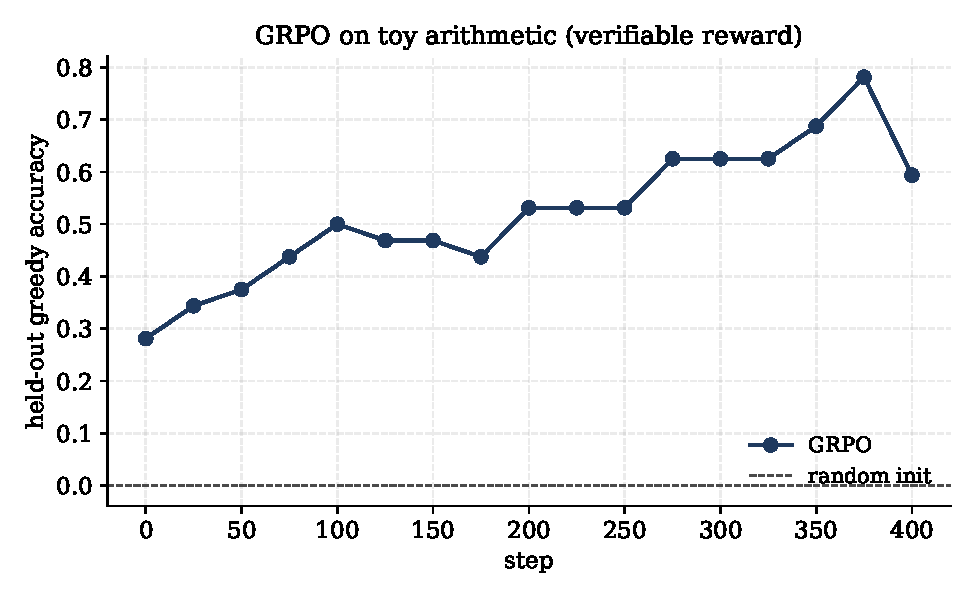
\includegraphics[width=0.85\linewidth]{figs/fig_grpo_accuracy.pdf}
\caption{Held-out greedy accuracy on the toy arithmetic task, evaluated
every 25 GRPO steps. The post-SFT initialisation lands near $0.45$;
500 GRPO steps push it to $\sim 0.65$.}
\label{fig:acc}
\end{figure}

\begin{figure}[t]
\centering
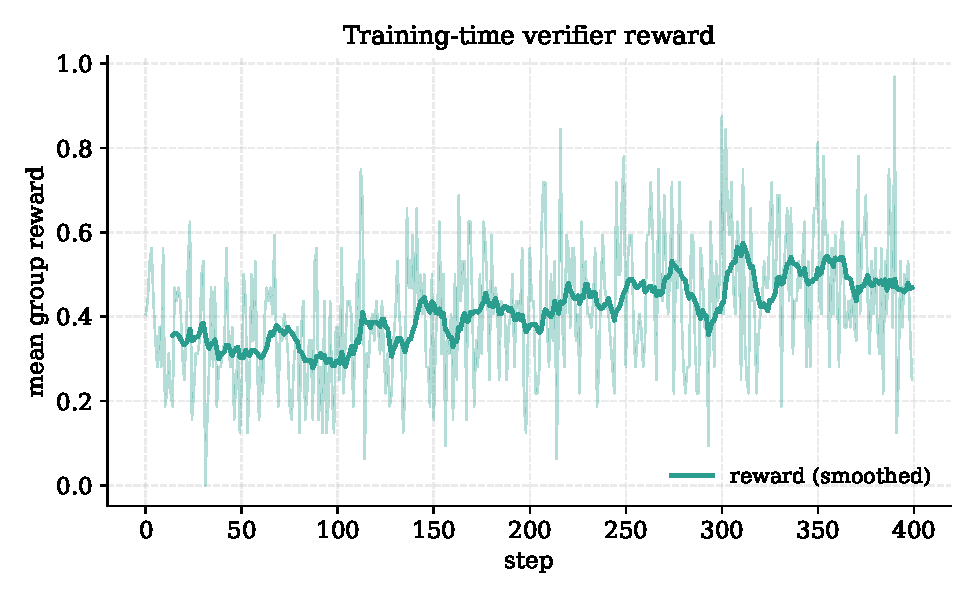
\includegraphics[width=0.85\linewidth]{figs/fig_grpo_reward.pdf}
\caption{Training-time mean group reward (raw and 15-step smoothed).
Reward is the binary verifier output. The variance is consistent with
the $p(1-p)$ Bernoulli bound at $p \sim 0.65$.}
\label{fig:reward}
\end{figure}

\section{What changes if we drop SFT?}

If we set \texttt{sft\_warmup\_steps=0} the GRPO curve sits flat at zero:
the verifier never fires, the group baseline is always zero, the advantage
is identically zero, and the gradient is zero. This is the standard
\emph{cold-start} pathology of RLVR. DeepSeek-R1-Zero famously bypassed it
on a large base model; for tiny models, a short SFT bootstrap is the
canonical fix.

% ===========================================================================
\begin{safetyangle}
\textbf{Failure modes specific to RLVR.}
\begin{enumerate}\setlength{\itemsep}{2pt}
  \item \emph{Verifier spec-gaming.} A code-verifier checking only that
        the unit tests pass invites \texttt{import sys; sys.exit(0)}.
        Defence: require the program to compute the result; sandbox; run
        secondary verifiers that re-execute the test harness.
  \item \emph{Format reward hacking.} If you reward $+0.1$ for emitting
        \verb|####|, the model will emit \verb|####| at the start of
        every line. Defence: only reward the format pattern when it is
        followed by a correctly parsed answer.
  \item \emph{Brittle math regex.} \texttt{r"\textbackslash d+"} matches the year
        ``2024'' inside an explanation. Defence: parse the final line,
        not the whole completion; use \texttt{sympy} equivalence rather
        than string equality.
  \item \emph{Distributional narrowing.} Pure RLVR shrinks the policy
        onto the verifier-rewarded distribution and forgets unrelated
        skills. \textsc{Tülu-3} mixes RLVR with a small DPO stream; many
        recipes keep a $\beta \ge 0.01$ KL anchor to the SFT model.
  \item \emph{Length bias.} The vanilla GRPO loss systematically favours
        shorter completions because of its $1/|y|$ normaliser; Dr.~GRPO
        and DAPO drop that divisor, and Kimi K1.5 adds an explicit length
        penalty.
\end{enumerate}
The safety analogue to \emph{Theorem~\ref{thm:rloo-unbiased}} is sobering:
the baseline subtraction is correct in expectation, but the empirical
average of LOO advantages over the policy's own samples can drift by
many standard deviations when the verifier rate is low --- exactly the
``rare-positive'' regime that triggers reward-hacking incentives. See
week~21 for the Gao~2022 over-optimisation scaling laws.
\end{safetyangle}

% ===========================================================================
\begin{matching}
\textbf{Process rewards as interview-stage signals.}
Insurance-broker matching (synthetic insurance) and candidate-job matching (synthetic ATS)
both involve a sequence of partial outcomes before a terminal one: in ATS,
\textsl{shortlist} $\to$ \textsl{interview-1} $\to$ \textsl{interview-2}
$\to$ \textsl{offer} $\to$ \textsl{hired}. A pure ORM reward (``did they
get hired?'') is sparse and slow. A PRM aggregator (the
\texttt{exercise\_7} solution in this week) lets the policy learn from
intermediate signals --- a candidate cleared interview-2 is informative
even if they ultimately declined the offer.

The matching analogue of Math-Shepherd's automatic PRM is: bootstrap the
step labels by Monte-Carlo from historical outcomes. ``This shortlist
profile predicts $70\%$ hire-rate'' becomes the step reward, the way
``this proof step continues to a correct final proof in $70\%$ of
rollouts'' becomes the step label in PRM800K.

\textbf{Practical caveat.} PRMs expand the gameable surface --- a
candidate-ranking policy can learn to satisfy the
``shortlist-stage signal'' (resume keywords) without improving downstream
hire rate. The pattern is identical to RLVR format hacking; see
week~21 for the mitigation toolkit.
\end{matching}

% ===========================================================================
\chapter{Exercises}

See \texttt{workbook.ipynb} for fully spelled-out cells with hints; the
summary list:

\begin{enumerate}\setlength{\itemsep}{2pt}
  \item[\textbf{\textcolor{rlteal}{$\bigstar$}}]
        Implement \texttt{extract\_final\_number} matching the GSM8K
        \verb|####| convention.
  \item[\textbf{\textcolor{rlteal}{$\bigstar\bigstar$}}]
        Implement the RLOO advantage from scratch and prove it is mean-zero.
  \item[\textbf{\textcolor{rlteal}{$\bigstar\bigstar$}}]
        Implement GRPO with and without standard-deviation normalisation
        (Dr.~GRPO) and reproduce the variance plot
        (Figure~\ref{fig:variance}).
  \item[\textbf{\textcolor{rlteal}{$\bigstar\bigstar$}}]
        Empirically confirm Theorem~\ref{thm:rloo-varred} on Bernoulli rewards.
  \item[\textbf{\textcolor{rlteal}{$\bigstar\bigstar$}}]
        Implement the unbiased k3 KL estimator and show it is non-negative
        across $10^4$ Monte-Carlo trials.
  \item[\textbf{\textcolor{rlteal}{$\bigstar\bigstar$}}]
        Code the PPO-clipped surrogate on a single token and sketch the
        loss landscape as a function of the importance ratio.
  \item[\textbf{\textcolor{rlteal}{$\bigstar\bigstar$}}]
        \emph{Matching-themed.} Implement three PRM aggregators
        (\texttt{min}, \texttt{mean}, \texttt{prod}) and discuss which is
        appropriate for the ATS interview-stage analogue.
  \item[\textbf{\textcolor{rlteal}{$\bigstar\bigstar\bigstar$}}]
        \emph{Open-ended.} Design a shaped reward with a format bonus,
        train with GRPO, and quantify the format-hacking failure mode by
        plotting ``rate of any-number-emitted'' vs ``rate of
        correct-number-emitted''.
\end{enumerate}

% ===========================================================================
\chapter{Further reading}

See \texttt{extended\_reading.pdf} for the curated five papers (DeepSeekMath,
RLOO, Dr.~GRPO, DeepSeek-R1, PRM800K). Section~3 of
\texttt{research/llm\_rl\_sota.md} carries the broader 2024--2026 dossier;
the verifier-design checklist in section~4 of that file is what we
operationalised above.

\end{document}
